\documentclass[11pt, a4paper, copyright, gdm]{google}

\usepackage{url}
\usepackage{tikz}
\usepackage{csquotes}
\usepackage{CJKutf8}
\usetikzlibrary{positioning}

\usepackage[
    backend=biber,
    style=numeric-comp, %
    sorting=none,       %
    %
    giveninits=true, 
    uniquename=init,
    natbib=true,
    maxbibnames=99,   %
    maxcitenames=2,   %
    mincitenames=1    %
]{biblatex}

\DeclareSourcemap{
  \maps[datatype=bibtex]{
    \map{
      \step[fieldset=primaryclass, null]
    }
  }
}

%
\DeclareNameAlias{sortname}{given-family}

%
\setlength{\bibitemsep}{0.5\baselineskip} %

%
\setlength{\bibhang}{15pt}

\RequirePackage[
  colorlinks=true,
  allcolors=blue,
  bookmarks=false,
  pdftitle={AI Co-Mathematician Chinese Translation},
  pdfauthor={Daniel Zheng et al.}
]{hyperref}
\usepackage[capitalize]{cleveref}

\addbibresource{main.bib}
\defbibheading{bibliography}{\section*{参考文献}}

%
\DeclareNameAlias{sortname}{given-family}

%
\setlength{\bibitemsep}{0.5\baselineskip}

%
\setlength{\bibhang}{15pt}

%
\newboolean{USECARTOON}
\setboolean{USECARTOON}{false} %

%
\newcommand{\usescreenshot}[2]{%
  \ifthenelse{\boolean{USECARTOON}}{%
    \includegraphics[#1]{assets/screenshot-#2-CARTOON.jpeg}%
  }{%
    \includegraphics[#1]{assets/screenshot-#2.png}%
  }%
}

%
%

%
\uselogo{} 

%
\title{{AI 协同数学家：用智能体 AI 加速数学家研究}}
\AtBeginDocument{\fancyhead[C]{\footerfont AI Co-Mathematician Chinese Translation}}
\linespread{1.25}

%
%
\correspondingauthor{dhhzheng@google.com, pushmeet@google.com}

%
\reportnumber{249243} %

%
%
%
%
\renewcommand{\today}{2026-05-07}

%
\author[1]{Daniel Zheng}
\author[1]{Ingrid von Glehn}
\author[1]{Yori Zwols}
\author[1]{Iuliya Beloshapka}
\author[1]{Lars Buesing}
\author[1]{Daniel M.~Roy}
\author[1]{Martin Wattenberg}
\author[1]{Bogdan Georgiev}
\author[1]{Tatiana Schmidt}
\author[1]{Andrew Cowie}
\author[1]{Fernanda Viegas}
\author[1]{Dimitri Kanevsky}
\author[2]{Vineet Kahlon}
\author[1]{Hartmut Maennel}
\author[1]{Sophia Alj}
\author[1]{George Holland}
\author[1]{Alex Davies}
\author[1]{Pushmeet Kohli}

%
\affil[1]{\thepa{}{}}
\affil[2]{Google}

\renewcommand\Authands{, and }


%
\newcommand{\user}[1]{\emph{#1}}

\begin{abstract}
我们介绍 AI 协同数学家，这是一个面向数学家的工作台，使数学家能够以交互方式借助 AI 智能体推进开放式研究。AI 协同数学家针对数学工作流中探索性、迭代性的现实进行优化，提供覆盖构思、文献检索、计算探索、定理证明和理论构建的整体支持。通过提供一个异步、有状态的工作空间，系统可以管理不确定性、细化用户意图、跟踪失败假设，并输出原生数学产物，从而贴近人类协作工作流。在早期测试中，AI 协同数学家帮助研究人员解决开放问题、识别新的研究方向，并发现被忽视的文献参考。除了展示一种高度交互的 AI 辅助数学发现范式外，AI 协同数学家还在困难问题求解基准上达到当前最优结果，其中在 FrontierMath Tier 4 上得分 48\%，这是所有已评测 AI 系统中的新高。
\end{abstract}

\begin{document}
\begin{CJK*}{UTF8}{gbsn}

\maketitle

\section{引言}

数学研究是一个多维、复杂且高度迭代的过程。
虽然公开发表的记录几乎完全建立在打磨过的严谨证明之上，但人们早已认识到，数学家的日常工作包含许多传统上不会呈现在公众视野中的活动 \citep{polya1954, lakatos1976, epstein1992}。
最终形式化表达的下方，是一个高度探索性的过程：最初的直觉会被检验，反例会被发现，核心定义和证明都会持续经历反驳与修订的循环。

近些年，AI-for-mathematics 的能力迅速爆发，推动该领域沿多个不同维度快速扩展。
在自主数学推理方面，从 Minerva~\citep{lewkowycz2022minerva} 等早期系统以及随后大量工作
\citep{taylor2022galactica,azerbayev2023llemma,yue2023mammoth,shao2024deepseekmath,mistral2024mathstral,yang2024qwen25math,lu2024aiscientist,deepthink2025,he2025skywork,yamada2025aiscientistv2,liu2025deepevolve,zimmer2026agentic} 出发，该领域如今已经推进到 Aletheia~\citep{feng2026} 这样的自主研究系统突破。
在探索式搜索方面，AlphaEvolve \citep{romeraparedes2024, novikov2025} 及其启发的系统 \citep{cemri2026adaevolve,sharma2025openevolve,lange2025shinkaevolve} 让研究人员能够通过连续、可引导的演化运行发现新的算法和结构。
在形式化数学方面，AlphaProof \citep{hubert2025}、相关系统 \citep{song2024leancopilot, wang2024legoprover, ren2025deepseekproverv2, lin2025goedelproverv2, li2025lips, chen2025seedprover, wang2025kimina, hariharan2026milestoneformalizationspherepacking, li2024hunyuanprover, jana2025proofbridge, chen2026parity, liu2026numina, deltredici2025axprover}，
以及 Aristotle \citep{harmonic2025aristotle} 等交互式环境，已经把强化学习和语言模型深度整合进可验证数学和开源证明助手。
%
与此同时，
%
当前支撑商业聊天界面的推理扩展模型，已经把巨大的解题能力直接交到数学家手中。

然而，对这些系统的一线使用经验表明，数学研究中仍有一个关键维度支持不足：如何把这些能力编排进长期、有状态、协作式的工作流。
日常数学工作很少只是孤立查询或计算机辅助证明的序列；它涉及管理不确定性、综合分散文献、起草并修订中间产物，以及在数天或数周内跟踪复杂且分叉的假设。

由于标准聊天界面天然短暂，而专门引擎又缺乏更宽广的上下文，研究人员不得不亲自充当连接组织，把对话式头脑风暴、形式化证明器和计算脚本手动串联起来。
软件开发者越来越依赖 AI 驱动的编码环境来提供这种编排能力，但这些工具本质上是为代码生命周期优化的，而不是为数学特有的抽象、证明和产物优化的。
若要真正加速发现，我们认为 AI-for-mathematics 的下一阶段必须聚焦这一缺失的编排维度，以原生方式支持数学活动完整而混乱的现实。

为了理解如何为这些活动构建原生环境，我们可以更深入地观察软件工程领域。
近期进展，例如 Google Antigravity \citep{google2025antigravity}、Claude Code \citep{anthropic2025claudecode} 和 OpenAI Codex \citep{openai2025codex}，展示了人与智能体 AI 系统高效交互协作的变革潜力。
这些系统成功的原因之一，是既有软件工程实践已经体现了捕捉并加速迭代探索所需的范式。
设计文档等非正式软件规范允许智能体在预定义路径上长时间自主工作，持续测试流水线提供自动化验证流程，而版本控制则以人类专业人士熟悉的方式无缝跟踪并维护项目演化状态。
相比之下，数学家日常工作中的类似活动几乎没有被常规自动化。

\begin{quote}\em
    为了为数学建立这种缺失的智能体流程，我们介绍 AI 协同数学家：一个基于最新 Gemini 语言模型的工作台，使数学家能够以交互方式借助 AI 智能体推进开放式研究。
\end{quote}
AI 协同数学家提供一个有状态、交互式的工作空间，其中项目协调智能体会把复杂任务委派到并行工作流中，让用户能够指导并参与一个持续演化的研究过程，而不是等待端到端的自主执行。
与其他智能体系统一样，AI 协同数学家是一个可与标准商业语言模型搭配使用的框架，并不依赖任何定制模型行为或训练。

重要的是，AI 协同数学家的设计目标是补充而非取代现有前沿方法。
通过建立这种有状态架构，我们为强大的底层引擎铺路，使自主推理器如 AlphaProof 和 Aletheia，或演化迭代器如 AlphaEvolve，都能被动态部署到人类研究者的交互回路中。
虽然 AI 协同数学家目前仍处于有限初始发布阶段，但我们的目标是开发未来产品，使更广泛的人群能够使用这种交互范式。

本文余下部分将详细介绍 AI 协同数学家的理念和架构，并分享早期结果。
第 2 节概述我们面向交互式 AI 辅助数学的核心设计原则。
第 3 节通过一个具体流程演示把这些原则落到实践中，重点说明程序化硬约束和对抗性审阅循环如何阻止系统在棘手问题上走捷径，以及并行工作流如何支持多侧面研究。
第 4 节讨论 AI 协同数学家这类交互式数学智能体的评估策略。
第 5 节呈现早期定性结果，展示执业数学家如何使用系统引导开放式研究并生成可验证洞见。
第 6 节评估系统在静态问题求解基准上的表现，给出其底层能力的基线测量。
第 7 节描述我们在开发 AI 协同数学家时遇到的挑战与限制。
最后，我们将概述对 AI 辅助数学下一时代的愿景。


\section{AI 辅助数学的设计原则}

我们设计的最高目标，是支持人类数学家完成他们自己的工作。
正如 \citet{Thurston1994} 的著名论述，数学从根本上说是一项旨在推进人类理解的社会事业，而不只是一台生成形式化证明的机器。
要真正加速数学家，AI 工具必须融入这种以人为中心的现实。
为此，AI 协同数学家被构建为捕捉专业数学工作流中持久存在的方面，同时务实地处理当前 AI 推理的优势与弱点。
我们的设计既基于关于数学实践的历史叙述，也基于我们观察和改进以往数学发现系统，尤其是 Google 内部系统的经验。
我们依靠七项核心原则来指导设计：

\begin{description}
    
\item[接纳证明之外的数学活动：] 真正的数学发现包含定理证明之外的复杂活动组合，例如反复细化研究问题、梳理文献、头脑风暴，以及进行大量计算和数值模拟来建立直觉，等等。
\citet{putnam1975} 认为，把数学还原为孤立的逻辑形式主义，会忽视这门学科深刻的准经验现实；我们的设计有意反映并支持这种整体、多模态的现实，而不是只围绕最终定理证明建立索引。

\item[支持意图的迭代细化：] 在许多领域，用户从一开始就清楚知道自己想要什么。
但在数学中，发现过程高度依赖持续迭代与细化。
正如 \citet{polya1954} 在关于似然推理的工作中所展示的，提出正确问题往往需要大量启发式猜测才能起步。
Georg Cantor 曾说：“在数学中，提出问题的艺术应当被视为比解决问题更有价值” \citep[p.~27]{dauben1979}。
AlphaEvolve 等系统的经验也印证了这一点：数学家会投入大量精力主动迭代到底该聚焦哪个问题，在扩展之前先用较小运行或相关问题进行测试 \citep{romeraparedes2024, novikov2025}。
我们设计了一个灵活界面，支持多条探索路径，使用户能够顺畅地细化定义、问题和猜想。

\item[产出原生数学产物：] 研究数学家已经有标准化的工作方式。
AI 协同数学家并不输出短暂的聊天日志，也不急于生成过早打磨的论文，而是把流程集中在一份持续演化的“工作论文”周围。
在传统工作流中，起草和批注会帮助数学家建立对项目的严谨心智模型，准确知道哪些部分已经稳固、哪些部分还需要进一步关注。
由于自主推理系统可以在用户视野之外异步完成许多探索性工作，用户可能会失去这种自然形成的上下文。
为了帮助用户重建心智模型，我们的系统会跟踪研究的演化状态，并通过行内文本和页边注进行可视化。
系统明确提供上下文，例如某项具体主张的来源，或某个已起草引理存在争议的程度，从而以数学共同体完全原生的格式呈现 AI 底层流程。

\item[支持异步交互与灵活引导：] 数学研究很少是线性过程。为了贴近这一点，系统并不是单个对话聊天机器人，而是一个异步团队。
在底层，一个消息系统允许多个专门智能体并行工作。
由于这些智能体异步运行，系统可以为一个问题分配可观的计算资源，同时不阻塞用户，使重计算和持续交互能够共存。

当系统“思考”时，用户不会被锁在外面；用户可以在任何时候直接与中央项目协调智能体沟通，以介入、绕过当前约束，并引导正在进行的研究。
这种协作也是双向的：如果智能体停滞，项目协调智能体会透明地标记障碍，并请求人类协助来帮助系统解除阻塞。

\item[通过渐进披露管理认知负荷：] 当用户和 AI 智能体协同探索多条并行路线、从死路回退、并复用中间结果时，复杂研究会变得难以掌控。
如果高层策略（例如“尝试不动点方法”）与多个后台智能体的低层执行日志（例如“我们必须验证第 40 行的可测性”）混在一起，一条冗长且无结构的聊天记录很快会变得不可用。
为了控制向数学家披露的信息量，我们的协作界面采用渐进披露，通过镜像智能体层级本身来把高层意图与低层执行分离。
默认情况下，用户主要与项目协调智能体交互，由它过滤专门智能体沙箱中的低层执行 chatter。
不过，系统始终允许用户按需深入查看任何并行智能体活动的细粒度细节。

\item[跟踪、管理并传达不确定性：] 数学发现要求很高的严谨标准，一个有缺陷的引理或幻觉出来的参考文献就可能破坏整篇论文。
由于基础模型的推理能力容易出现不可预测的短板，其零样本输出会给一个要求精确的领域引入基本不确定性。
系统架构并不隐藏这种摩擦，而是围绕这种不确定性的生命周期来设计。
它通过维护详细版本历史来\emph{跟踪}不确定性，这一历史主要供智能体使用，也可供用户查看，用于监控主张如何演化或被质疑；它通过用计算换取验证来\emph{管理}不确定性，例如持续审阅、数值模拟和系统化引文检查；它还会在审阅过程卡在论证的具体部分时识别这种状态，从而\emph{传达}摩擦。
通过使用行内高亮和页边注把用户注意力引向这些停滞段落，系统突出工作论文中值得人类进一步细查的区域。
把不确定性视为一个需要编排的核心变量，而不是简单的错误状态，使系统能够从本质上不可预测的模型中综合出更稳健的数学输出。


\item[保留失败探索的历史：] 在数学研究中，知道什么行不通往往和知道什么行得通同样重要。
虽然智能体会被配置为绕开障碍，但系统接受特定目标或并行工作流可能以失败告终。
架构不会静默重启或擦除这些失败尝试的历史，而是把死路视为一等的永久结果。
保存项目历史中的这种“负空间”，对处理困难数学问题至关重要。
通过维护失败目标和穷尽策略的持久记录，系统为用户和 AI 提供上下文，使二者能够基于这些失败本身协同制定新的、更有信息量的工作流；这也呼应了反驳是数学进步之根本的观点 \citep{lakatos1976}。

\end{description}

%

\section{实践中的 AI 协同数学家：流程演示}

为了展示我们的设计原则如何在实践中体现，本节演示一次具有代表性的协同数学家原型使用会话。

在这个场景中，一位数学家探索计算几何中的一个开放问题：证明某种“沙发”面积的上界，该沙发可以绕过左手和右手两种直角拐角。
这是 \citet{moser1966moving} 首次提出的问题的一个变体，其下界在近期将 AlphaEvolve 应用于数学优化问题的工作中被探索过 \citep{georgiev2025}。

系统并不作为标准对话聊天机器人运行，而是提供一个关联的“工作空间”，项目的所有信息都存放于其中。
这个工作空间由一个智能体层级来操作，智能体会把工作写入共享文件系统，并通过内部消息系统通信。
用户向顶层项目协调智能体提供输入并讨论想法，该协调智能体把工作委派给链条下游的其他智能体，依此类推。
与人类组织类似，我们观察到，为了让群组正常运转，智能体在遇到问题时需要可用的沟通线路和清晰的升级路径。
\cref{fig:org_chart} 给出了智能体组织的近似图示。

\clearpage
\begin{figure}[t]
\centering
 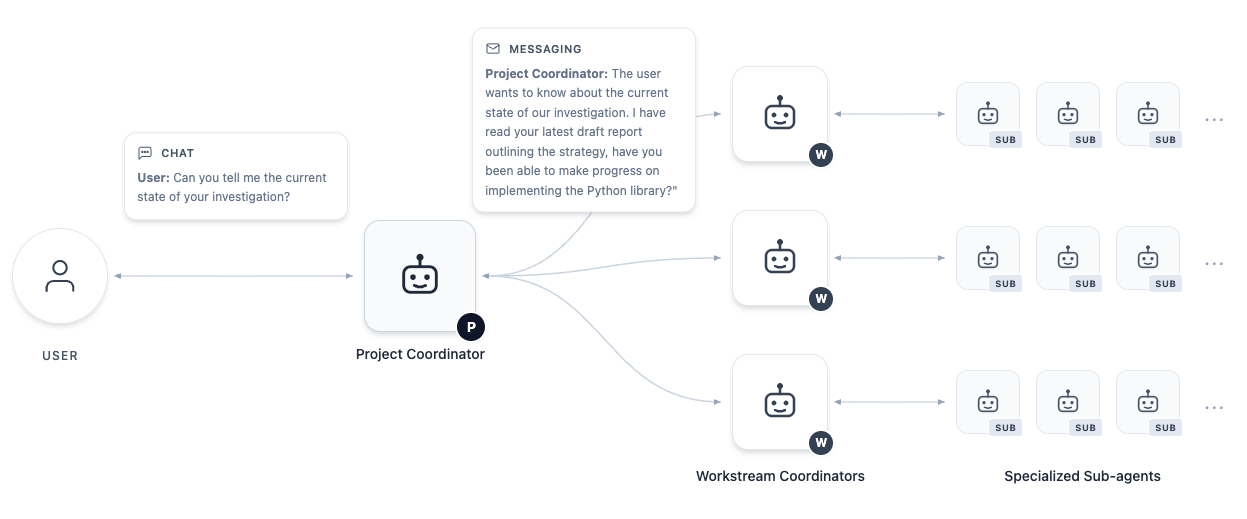
\includegraphics[width=\columnwidth]{assets/comath_org_chart.png}
\caption{典型 AI 协同数学家工作空间中智能体组织的简化图。箭头表示标准通信路径，这些路径用于收集用户所需的信息，并分发来自用户的指令。}
\label{fig:org_chart}
\end{figure}

\subsection{初始探索}

\begin{figure}[t]
\centering
 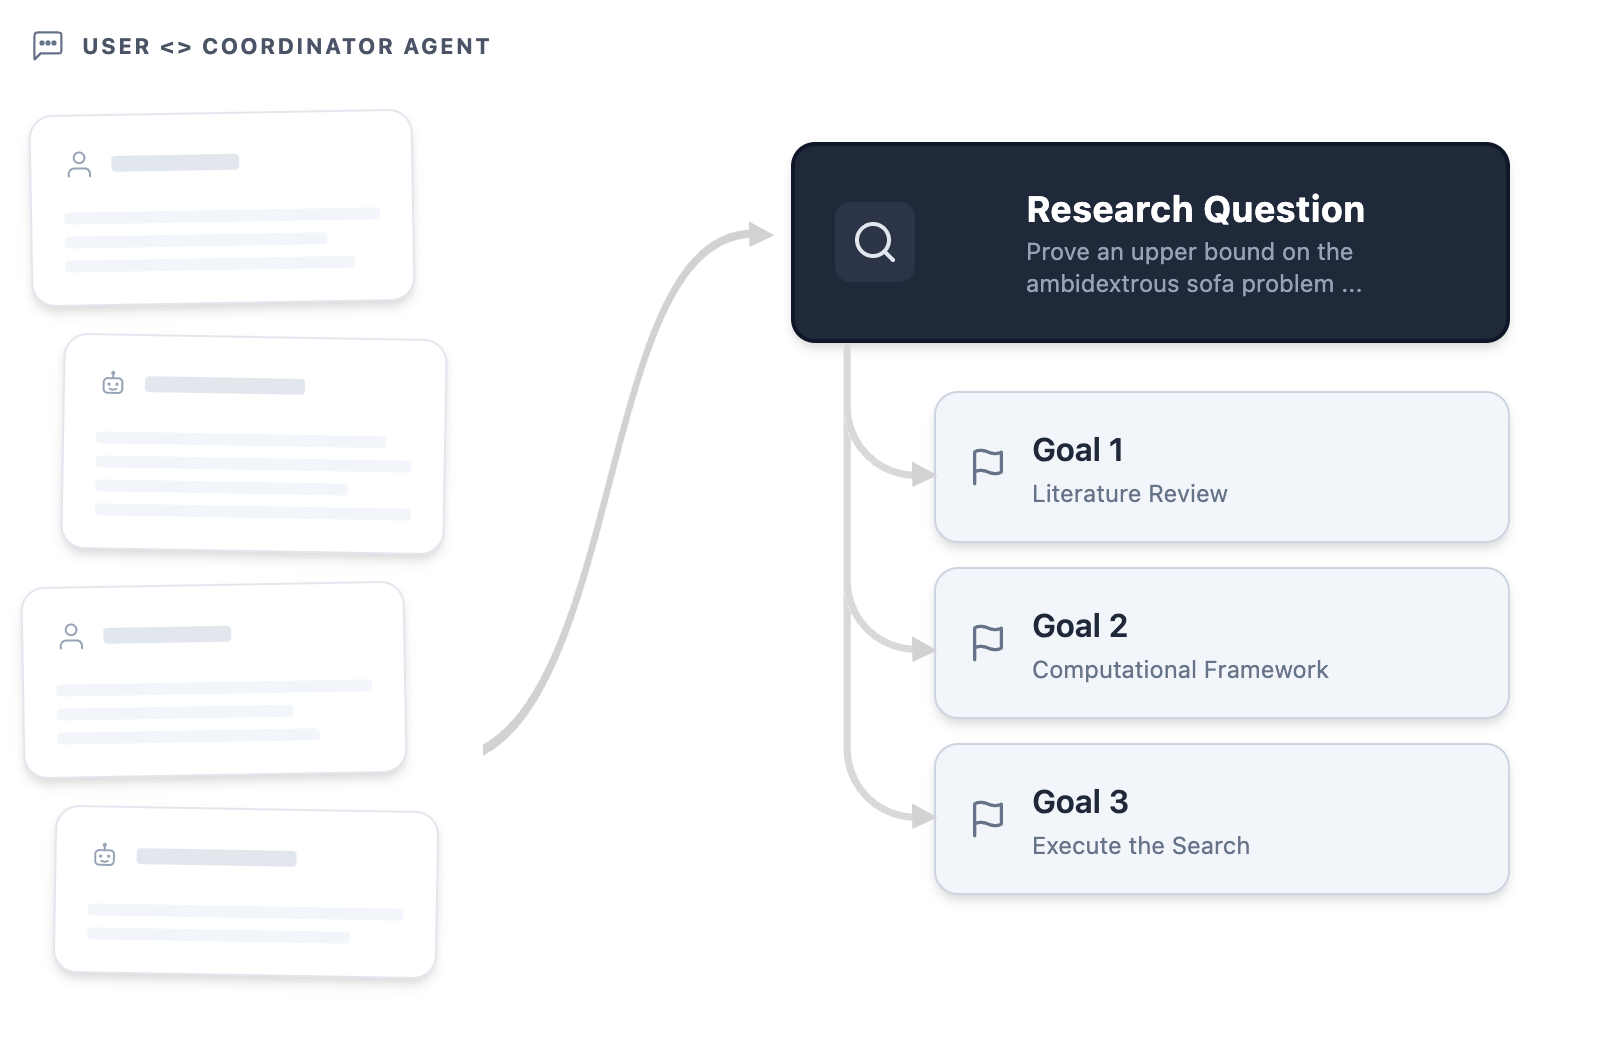
\includegraphics[width=0.7\columnwidth]{assets/intake_figure.png}
\caption{在初始探索阶段，用户与项目协调智能体之间的对话会形成一个经用户批准的研究问题和项目目标。}
\label{fig:initial_conversation}
\end{figure}

标准零样本 LLM 要求用户在一开始就给出完美提示。
为了体现我们支持意图迭代细化的原则，AI 协同数学家从一个交互式入门阶段开始，帮助用户形式化自己的意图。

在这个例子中，用户通过向聊天界面上传一篇近期论文 \citep{georgiev2025} 和一些上下文来启动会话：\user{“我想建立一个项目，看看我们是否能够证明这篇论文讨论的移动沙发问题变体的一些上界。”}

顶层项目协调智能体并不会立即开始求解。
相反，它开启对话并充当讨论对象，在聊天中回复：\user{“从文本看，Baek 已经证明 Gerver 的下界对经典沙发问题是紧的。不过，另外两个变体的上界仍然开放：\ldots{} 你想特别聚焦其中一个，还是两个都做？你的目标是证明某个具体下界是紧的，还是只要建立任何新的、严格的上界？”}

当用户澄清后，项目协调智能体会形式化它对项目中心问题和高层目标的理解，并把它们呈现给用户。
用户详细阅读这些提案后，要求修改目标措辞，项目协调智能体随即更新。
此时用户正式批准目标，使项目协调智能体能够进入项目的下一阶段（\cref{fig:initial_conversation}）。
通过把初始交互视为对话，系统确保下游资源被导向数学家实际且已经细化的意图。


\subsection{研究分支}

\begin{figure}[t]
\centering
 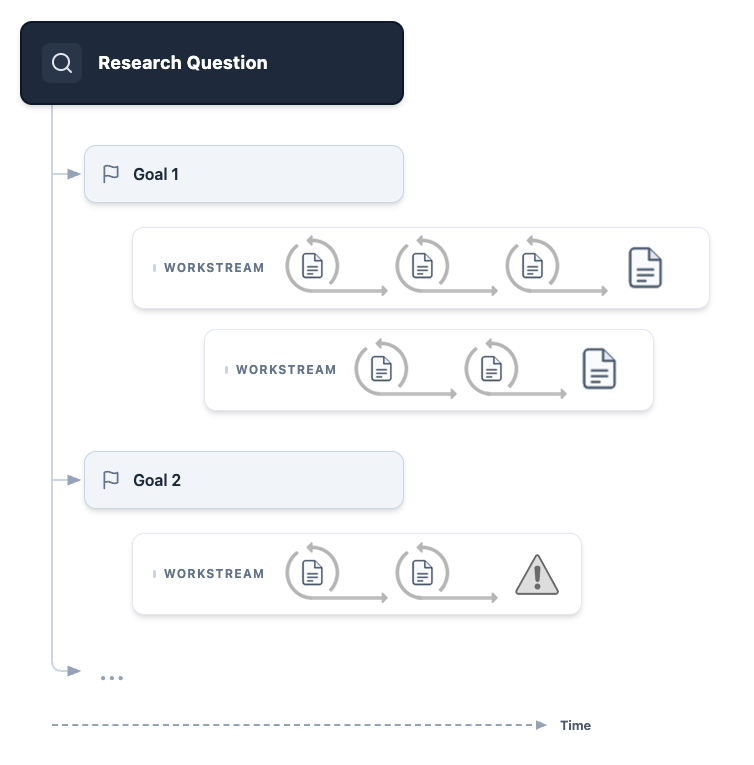
\includegraphics[width=0.5\columnwidth]{assets/multiple_workstreams_warning.png}
\caption{一旦研究问题和目标被定义，项目协调智能体就会调度工作流，以推动目标进展。每个目标可以关联多个工作流，也可以在调查过程中的任何时刻添加额外工作流，例如响应用户的特定请求。每个工作流都力图产出一份经过完整审阅的报告，附带附件和外部参考，同时还会提供增量报告，供用户在工作仍在进行时判断部分进展。工作流可能由于多种原因无法完成任务；在这种情况下，系统会在增量报告旁向用户显示醒目的警告。}
\label{fig:multi_workstream}
\end{figure}


\begin{figure}[t]
\centering
 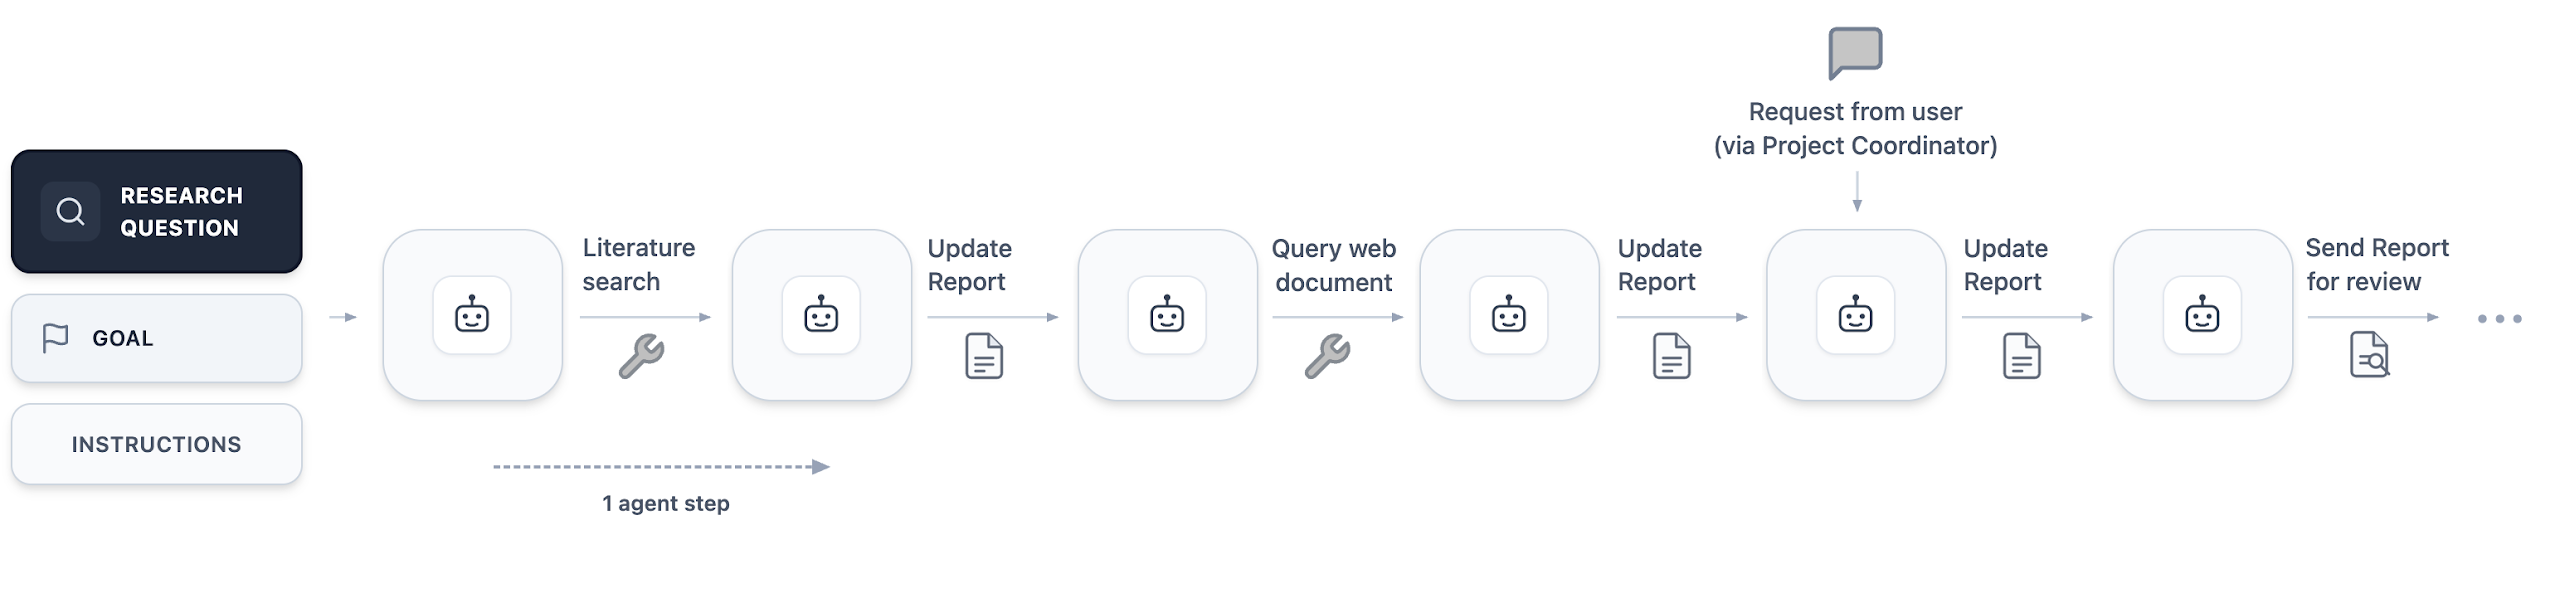
\includegraphics[width=\columnwidth]{assets/workstream_figure.png}
\caption{单个工作流由工作流协调智能体采取的一系列动作组成，这些动作可能会更新项目状态和/或用户界面。在这个简化示例轨迹中，工作流协调智能体先执行文献搜索，再执行一次具体 Web 查询，并在每次行动后用发现更新报告。随后，它收到来自项目协调智能体的消息，传达用户请求，于是进一步更新报告。工作流协调智能体接着把最新报告送审。如果审阅成功通过，协调智能体即可把工作标记为“完成”。}
\label{fig:workstream}
\end{figure}

目标定义完成后，系统通过渐进披露管理用户认知负荷：项目协调智能体把工作委派给并行工作流，每个工作流都关联一个预先批准的目标，并由各自的工作流协调智能体管理（\cref{fig:multi_workstream}）。作为输入，工作流协调智能体会收到已批准研究问题的陈述、所选目标，以及项目协调智能体选择提供的任何具体指令。
每个协调智能体会执行一条线性动作序列，其中可能包括委派给专门子智能体（\cref{fig:workstream}）。
这些工作流的多样性凸显了系统接纳证明之外数学活动的能力。
目前，我们的专门子智能体基于标准 LLM 调用（包括 Gemini Deep Think），并未使用 AlphaEvolve、AlphaProof 或 Aletheia 等高级研究系统，但我们会说明在流程中哪些位置自然适合它们发挥价值。

这里我们描述一个场景：项目协调智能体为每个目标启动一个工作流；但也可以为每个目标定义多个工作流，或者让某些目标在其依赖工作完成之前暂不填充工作流。

\textbf{目标 1：文献综述：} 一个工作流协调智能体委派给专门的文献综述子智能体。
它利用我们计算密集型的搜索工具，发现了包含以往沙发问题上界所用机制的关键论文。
有了重要参考文献指针后，它使用具体 Web 和文献访问工具直接查询这些文献，以识别关键结果的精确陈述和证明。

\textbf{目标 2：计算框架：} 另一个工作流协调智能体处理设计所需计算框架的任务。
基于以往文献中的策略，工作流协调智能体首先设计计算框架的高层逻辑，并使用子智能体创建工具派发 Gemini Deep Think 来证明该框架确实能够给出所需的严格上界。
一旦这一点被证明，它再使用另一个子智能体创建工具来创建编码智能体，并指示其实现所需 Python 库及相应测试和演示案例。
随着这些智能体提供状态更新，工作流协调智能体会异步更新面向用户的工作流报告，写入证明细节，并提供关键代码文件链接。

现有系统中的所有证明都只是非形式化证明，但加入 AlphaProof 这样的形式化证明器，将有助于提高证明正确性的可信度，前提是相关命题能够用现有形式化数学库陈述并证明。
或者，使用 Aletheia 这样更强的非形式化证明系统，也会显著增强系统能力，但会带来相应的计算成本。

\textbf{目标 3：执行搜索：} 最终的分支定界搜索会在另一个工作流中执行，该工作流由项目协调智能体在计算框架工作流成功完成后创建。
共享文件系统允许这个工作流协调智能体导入上一工作流开发的库，然后使用并行代码执行工具，把搜索扩展到单个脚本之外。
并行代码执行请求会在独立云机器上运行，避免要求用户配置或访问本地集群。
搜索结果被汇总到一个文件中并附加到工作流报告，同时摘要信息和结论被写入正文。

在当前原型中，这类计算搜索由标准智能体原语组合执行；但加入 AlphaEvolve 等演化搜索算法，将为这类优化与搜索流程提供更强大的引擎。

\subsection{交互式引导与硬约束}

当被要求解决困难研究问题时，标准 AI 智能体常常会寻找无效捷径、幻觉出引理、含糊处理细节，并过早宣称成功。
AI 协同数学家的一个定义性技术特征，是应用硬性程序化约束来防止这些失败模式，并结合用户的主动人工引导。

在计算探索期间，如果搜索空间爆炸，最初提出的朴素回溯方法可能会失败。
在这种情况下，编码子智能体受到严格规则约束：只有在测试通过，并且审阅智能体接受代码和测试中黄金值的有效性之后，它才能把代码标记为完成。
由于审阅智能体反复拒绝失败代码，工作流协调智能体被阻塞。
系统不会静默重启，而是把这次失败探索作为共享文件系统中的持久记录保留下来，供项目协调智能体读取。

在被迫管理并披露其不确定性的情况下，项目协调智能体会向用户呈现警报，并在聊天中明确请求帮助：\user{“我们最初的搜索实现效率不足，无法找到所需结果，而且文献中也没有很多其他例子。你是否有数学直觉，知道可以应用哪种更好的剪枝策略？关于当前方法的更多细节见下列文档。”}

关键在于，用户在智能体工作时不会被锁在外面。
通过聊天界面，用户阅读项目协调智能体的更新，并主动引导项目：发送消息提出一个拓扑剪枝启发式方法，同时指示协调智能体创建额外工作流，在当前工作仍在进行时调查新的界定策略。

\subsection{最终输出}

在用户引导系统越过计算瓶颈之后，各工作流完成了各自目标。
不过，最终输出不是一条短暂的聊天消息。
%
每个工作流协调智能体的主要输出，都是一份经过编译和审阅的 LaTeX 文稿；当用户打开该工作流时，这份文稿会被醒目展示。

为了产出自然的数学产物，我们要求协调智能体在这些文稿中满足具体标准：

\begin{description}
\item[阐释：] 草稿必须包含对研究过程如何导向结果的解释，而不只是最终结果本身。

\item[页边批注：] 文档使用页边注提供额外信息，明确把主张链接回工作空间。
一条注释可能写作：\user{[剪枝启发式来自用户建议；2.2195 的基线界来自 arxiv.org/abs/... 上的论文。]}

\item[内部链接：] 除外部文献外，文档还引用智能体创建的内部文档，让用户能够直接进入共享文件系统进行审计。

\item[审阅流程：] 报告在被标记为最终完成、工作流被完成之前，必须提交给论文审阅流程，由多个 AI 审阅智能体从内容和风格上进行细查；这些审阅智能体都具备交叉检查参考文献、代码输出以及逻辑正确性的工具和能力。
审阅智能体会在多轮审阅之间持续存在，从而形成一个报告不断被细化和改进的迭代过程，直到\textit{所有}审阅者都正式批准报告才结束。
为了避免无限循环，如果工作流协调智能体无法通过审阅流程，它可以把问题升级给项目协调智能体。
在这种情况下，工作流会被标记为未完成，并向用户清楚显示升级消息，使用户能够立即理解该报告可能仍含有未解决问题。
\end{description}

\section{交互式数学智能体的评估}
\label{sec:evaluation_paradigm}

历史上，AI-for-mathematics 的进展一直通过静态问题求解基准来衡量。
今天，该领域仍高度依赖这类基准，包括 IMO ProofBench \citep{luong2025imobench}、FrontierMath \citep{glazer2024} 和 PutnamBench \citep{tsou2024putnambench}；它们的前身 MATH \citep{hendrycks2021math} 和 GSM8K \citep{cobbe2021gsm8k} 在衡量早期 LLM 进展方面曾极具影响力。

然而，当前前沿系统已经在\textit{原始问题求解能力}上可证明地达到或超过专家人类水平 \citep[e.g.,][]{luong2025advanced, abouzaid2026proof}。因此我们认为，继续提高这一能力的边际价值正在下降，而 AI 辅助数学的进展如今至少部分受制于其他能力，这些能力反映了专业数学家更宽广的工作流。

这首先意味着，AI 系统应在更广泛的任务阵列上被测量。
DeepSearchQA \citep{gupta2026} 等用于通用事实查找的基准，以及 Hard2Verify \citep{pandit2025} 等用于竞赛数学证明找错的基准，都测量了数学研究过程中有精确对应物的能力。
但据我们所知，在专业研究数学场景下，还没有类似基准被开发出来。
随着 AI 系统进步，对这些辅助能力进行清晰测量，并在这些测量上取得改进，将变得越来越重要，以降低“锯齿状前沿” \citep{dellacqua2026navigating} 的严重性，以及人类驱动数学与 AI 驱动数学之间相关的阻抗不匹配。

更重要的是，我们认为 AI-for-mathematics 系统默认应被视为人在回路中的系统，并据此衡量进展和成就。
这呼应了我们的设计原则：系统的首要目的，是协助数学家完成他们的工作，而不是脱离他们独立取得成功。
在这一框架下，我们先呈现由数学家直接使用 AI 协同数学家所产生的结果（\cref{sec:early_results}），随后给出 AI 协同数学家静态问题求解表现的测量（\cref{sec:benchmarks}）。

\section{与数学家合作的早期结果}
\label{sec:early_results}

作为让交互式工具更广泛可用的努力的一部分，我们向少数专业数学家开放了 AI 协同数学家的访问权限，供他们用于自己的研究。
早期用户用 AI 协同数学家探索的使用场景范围很广，反映出它具有广泛适用性，并能融入标准研究工作流。
AI 协同数学家已经在若干场景中作为功能性辅助工具发挥作用，例如导航分散文献、进行数值实验，以及在多个数学领域获得证明。
本节余下部分展示若干使用案例，说明系统当前的实用性；这些案例来自近期有限发布中的用户。
需要说明的是，虽然许多用户与 AI 协同数学家的交互成功导向了新发现，但用户对该工具的反馈和满意度存在差异，也有其他用户认为它对自己的工作效果较弱。
我们会在第 \ref{sec:limitations} 节讨论其中一些挑战，并希望利用这些数学家的经验和反馈来指导未来基准构建和开发方向。

值得注意的是，这里展示的所有结果，都是数学家直接使用工具独立产生的，没有 GDM 研究人员的任何监督或干预。


\subsection{案例研究：一个 Kourovka 问题}


一位早期用户 M. Lackenby 使用 AI 协同数学家调查拓扑和群论中的若干问题。
他的工作解决了一个开放问题（Kourovka Notebook 中的问题 21.10）。\footnote{该问题询问每个有限群是否都承认所谓“just finite presentation”，即一种有限表示，删除任何关系后都会得到无限群。答案最终是肯定的。}
Lackenby 在这个案例中的过程，说明了“数学家在回路中”式交互的价值。

Lackenby 一开始只是输入问题陈述；系统确认其含义后，创建了两个独立工作流，一个尝试证明结果，另一个尝试反驳结果。
最先返回的是一个系统自身标记为不正确的“证明”：某个工作流写出了一个论证，但审阅智能体发现了缺陷。
然而，当 Lackenby 查看论文时，他意识到，尽管存在这个缺口，其中包含了他称为“真的非常非常聪明的证明策略”的内容。
进一步地，当他阅读审阅者对证明的批评时，他意识到：“等一下，我知道怎么补上这个缺口。”

他指出了一种修正论证的方法，系统随后能够写出一个完整且正确的证明。
最后，Lackenby 下载文档并进行了自己的修订，包括推广结果和添加例子，然后再次上传，并请求项目协调智能体创建一个工作流做最终审阅。
系统照做了，并在论文中发现两个小问题，他修复后形成最终版本。

这个案例的一个教训是，AI 与数学家之间的来回互动，对问题解决至关重要。
在 Lackenby 看来，这意味着“系统在用户熟悉该领域时效果最好”。
虽然有人可能把这看作限制，但他补充说：“让我让它解决一个我完全不懂的问题，有什么意义呢？”

\paragraph{智能体动作}

在幕后，该工作流的协调智能体：
\begin{itemize}
     \item 创建了一个编码子智能体，用于执行非 just-finite presentation 的计算搜索，并成功找到了两个例子。
     \item 分析这些例子，并进行文献搜索，以识别与其构造相关的理论，从而得到一种产生非 just-finite presentation 的一般方法。
     \item 注意到这并没有否定该猜想（因为群可能有多个表示，找到一个非 just-finite presentation 并不意味着它们都不是 just-finite），但决定以基于该论证形成的更尖锐猜想结束工作流，并把报告送审。
     \item 作为审阅流程的一部分，与审阅智能体展开来回讨论。
     在此期间，一个审阅智能体发现了一种可用于从正向证明该猜想的方法。
     \item 同意审阅者意见，并把工作流转向写出这一方法。
     经过进一步审阅，这导向了 Lackenby 后续补强并完成证明的草稿。
\end{itemize}


\subsection{案例研究：Stirling 系数}

另一位早期用户 G. B\'erczi 最初使用 AI 协同数学家处理一个问题，该问题涉及对称幂表示的 Stirling 系数行为。
具体而言，相关猜想假设在某个二项展开中，系数不仅严格为正，而且形成一个对数凹序列。

为了启动项目，B\'erczi 准备了一份简短笔记，介绍主题、猜想背景和已知方法。
这份入门材料还包含了从他先前使用其他系统（如 AlphaEvolve）进行实验中得到的建议方向。
虽然 AlphaEvolve 未能解决更高指标的情形，但它暗示了一个可能方向，用于恢复系数的归纳公式。
B\'erczi 把这一点写入文档，并在初始项目表述讨论中上传。
这种为问题提供深入、丰富背景的方式，被 B\'erczi 称为“结构化提出问题”，也是他在其他 AI 系统中发现有效的做法。

针对 B\'erczi 的问题，AI 协同数学家在独立工作流中为两个猜想建立了证明（目前仍在详细人工审阅中）。
它还为其主张以及对未证明猜想的调查提供了详细计算证据。
B\'erczi 指出，系统设计在多个方面提供了帮助。
不仅“绿色勾号”让任务进展易于跟踪，更重要的是，完成文档中的一条页边批注提示了一个关键洞见，使他能够在聊天界面中继续追问。
尽管如此，他也指出，与 AI 系统协作需要一定技巧，并说“现在如何使用它并不简单”，还建议“数学家如何使用这些模型，会造成很大差异”。

\paragraph{智能体动作}

两个关键工作流提供了声称的猜想证明。
为了说明工作流，在第一个工作流中，协调智能体：
\begin{itemize}
     \item 创建了一个编码子智能体，用于对展开式进行初始计算枚举，枚举规模控制在几分钟内合理可运行的范围。
     \item 从结果中观察到，按原陈述，该猜想在 $n = 1, 2$ 时为假，但对更大的 $n$ 似乎成立；同时还发现其原始证明策略无效。
     \item 使用 Gemini Deep Think 子智能体为更新后的猜想提出新的证明策略。
     该子智能体成功完成任务，说服了工作流协调智能体，随后也说服了审阅智能体。
\end{itemize}



\subsection{案例研究：Hamiltonian 系统中的一个引理}

第三位 AI 协同数学家的早期用户 S. Rezchikov 提出了他近期研究中遇到的一个技术子问题，主题是某类 Hamiltonian 微分同胚的扰动是否存在，并满足若干便利性质。

使用系统时，Rezchikov 与项目协调智能体讨论该问题，并提供了包含与问题陈述相关结果的补充论文，直到双方就任务的精确定义达成一致，并创建了一个工作流来尝试解决它。
该工作流生成的文稿包含一个关键引理及其优雅证明，经仔细检查后站得住脚，并实质性解决了 Rezchikov 提出的问题。
Rezchikov 也指出，在相同提示下，其他 AI 系统未能证明该结果；不过，如果没有多次采样尝试和受控条件，很难从这类单个实验中得出结论。

Rezchikov 还提出了两个观察，帮助说明系统价值。
一个是关于探索某条似乎行不通的路线：这里的增值在于系统让他比原本更快抵达死路。
用他的话说：“我本来可能很容易花一周时间幻想那里有什么，但现在我直接继续前进了。”
另外，他指出，正确证明的质量似乎相对较高：“从美感上说，我会把它的总体证明风格排在我用过的所有模型之首。”

这说明 AI 协同数学家可以帮助数学研究人员以一种自然融入其典型探索性研究工作流的方式探索想法。

\paragraph{智能体动作}

在这个案例中，工作流协调智能体：
\begin{itemize}
    \item 使用专门工具对相关问题中常用技术和陷阱进行文献综述，除 Rezchikov 已提供的性质外，还突出了一些需要注意的关键性质。
    \item 发起具体的后续文献查询，以理解这些要点的精确性质。
    \item 将问题陈述和关键上下文交给 Gemini Deep Think，后者生成了证明，包括关键引理；随后该证明被写入报告。
\end{itemize}


\section{问题求解基准结果}
\label{sec:benchmarks}

在论证了更宽能力测量的必要性后，我们也承认，问题求解基准目前仍是衡量 AI 系统数学表现的最佳可用客观指标。
本节讨论我们使用这类基准测量 AI 协同数学家表现的尝试。

由于 AI 协同数学家的设计方式是通过长篇报告传达结果，并在卡住时向用户提问，我们开发了一个自定义模式：在该模式中，系统除了初始问题外不能接收外部输入，并在用户聊天面板中返回一个单一最终答案。
这一模式实现的主要差异包括：
\begin{itemize}
    \item 绕过初始问题定义对话，并假设问题陈述中已经包含所有必要信息。
    \item 把单一项目目标硬编码为“解决该问题”。
    \item 
    \begin{minipage}[t]{\linewidth}
    引入固定时间限制；若项目协调智能体此前尚未给出最终答案，则时间到后必须给出最终答案。内部评估设为 24 小时，FrontierMath 设为 48 小时。
    大多数问题尝试会在该时间限制内较早完成，但对于缺乏人工干预的困难问题，系统偶尔会超过这一时长，尤其是在难以生成干净解答的情形中。
    \end{minipage}
\end{itemize}

作为一个长时间运行的智能体系统，与通常在这些任务上评估的基础模型相比，AI 协同数学家使用了相应更多的计算资源。
不过，虽然 AI 协同数学家的求解尝试没有显式推理限制，但系统被开发为足够高效，可以服务许多外部用户。
我们观察到，每次尝试使用的模型与工具调用数量，大体可与一次较长的 AI 辅助软件工程会话相比，这与其作为交互式智能体工具的主要使用场景相匹配。

\subsection{内部研究数学评估}

我们在一个内部基准上测试了 AI 协同数学家，该基准包含 100 道未泄漏的研究级数学问题，答案可通过代码检查，题目来自专业数学家。

在这些基准上，AI 协同数学家显著优于对 Gemini 3.1 Pro 模型的单次调用，也显著优于对 Gemini Deep Think 系统的单次调用（\cref{fig:benchmark}）。
如前所述，AI 协同数学家也使用更多计算：事实上，AI 协同数学家底层许多内部智能体都构建在 Gemini 3.1 Pro 之上，而证明智能体可以调用 Gemini Deep Think。

分析具体例子时，我们看到 AI 协同数学家不同特性的收益。

\begin{figure}[t]
\centering
 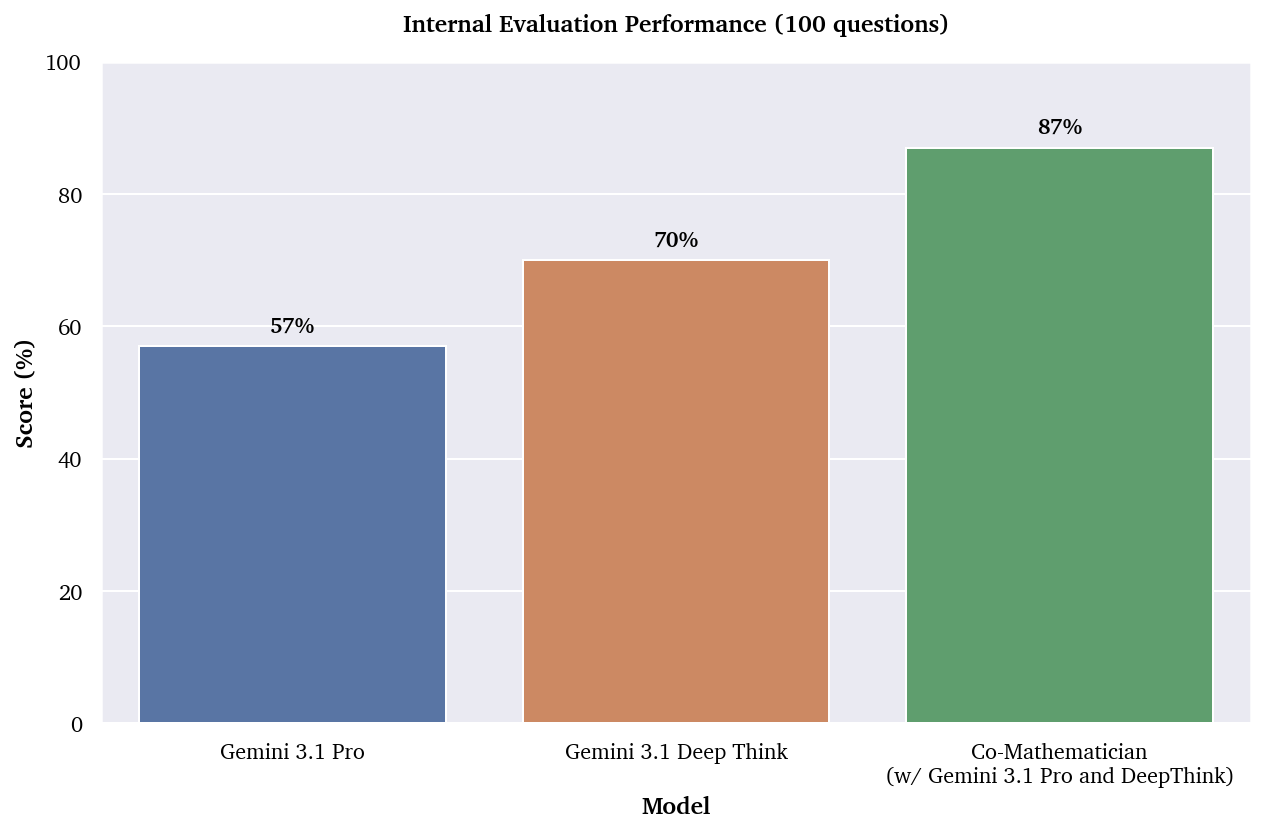
\includegraphics[width=0.85\columnwidth]{assets/eval_plot_overall.png}
\caption{Gemini 3.1 Pro、Gemini 3.1 Deep Think 与同样基于 Gemini 3.1 的 AI 协同数学家，在一个内部研究数学基准上的准确率得分。}
\label{fig:benchmark}
\end{figure}

%
在一个关于几何平铺的问题中，我们看到 AI 协同数学家成功把问题核心化约为一个布尔可满足性（SAT）问题，并使用 \texttt{PySAT} 库求解。
为了让这种表述成立，需要对核心问题做出若干非平凡改造；这种解法显然偏向于拥有持久文件系统和智能体式代码编写能力的系统。
虽然其他模型的评估框架允许执行代码，但它们很难开发和测试更复杂的库。
Gemini 3.1 Pro 和 Gemini Deep Think 都尝试对该问题给出纯理论解法，而在这个案例中，这是一项困难得多的任务。

%
在一个表示论问题中，AI 协同数学家使用其文献搜索工具，从相关论文中正确检索出精确的定理陈述，并将其应用于任务求解。
其他模型尝试应用更一般的定理；虽然这些定理与该主题领域相关，但如果无法访问文献以检查精确陈述，它们就不能把定理条件正确匹配到问题中的假设。

%
在一个兼具理论和计算方面的组合问题中，我们看到 AI 协同数学家把工作清晰拆分到多个工作流中，将解法的理论基础细化与代码开发分开处理。
在理论工作流中，执行抽查的审阅者指出了多个逻辑错误和不一致之处（类似其他模型犯下的错误），这些问题最终在工作流报告中被修正，使项目协调智能体能够整齐地组合各部分，给出正确解法。

\subsection{FrontierMath}

一个自然比较对象是外部 FrontierMath 基准 \citep{glazer2024}。
Epoch AI 在该基准的 Tier 4 上测试了 AI 协同数学家，使用的是上述最终答案模式。
用 Epoch AI 的话说，“这个极端层级包含 50 道问题，由教授和博士后设计为短期研究项目。它们被设计为难度超过 Tier 3，其中一些可能在未来数十年内仍不会被 AI 解决”。
来自主要提供商的前沿模型和系统会定期在 FrontierMath 基准上被测试。\footnote{最新结果和排行榜可见 \url{https://epoch.ai/frontiermath/tiers-1-4?tier=Tier+4}。}

这项评估以盲测方式进行，Epoch AI 可直接访问 AI 协同数学家的 UI，并自行输入问题、取回答案；系统开发者没有看到问题，也没有观察评估期间项目工作空间的状态。

AI 协同数学家在该基准上取得新高分：排除两个公开样例问题后，它在 48 道题中正确解决 23 道，准确率为 48\%。
值得注意的是，这相对 AI 协同数学家所基于的 Gemini 3.1 Pro 基础模型有显著提升，后者准确率为 19\%；这表明我们的并行调查分支、强制审阅循环和工具实现能够改善问题求解任务中的结果。
正确解决的问题中，有三道此前没有被任何已评测系统解决过；不过，AI 协同数学家也未能解决两个至少被一个先前系统解决过的问题。

与先前评估相比，一个重要差异是，FrontierMath 评估通常使用 Epoch AI 开发的标准智能体框架执行。\footnote{一个值得注意的例外是：Gemini 2.5 Deep Think 也通过 Web UI 评估，没有使用额外框架 \citep{epoch2025evaluatingdeepthink}。}
该框架提供 Python 解释器访问，但也对智能体轨迹中使用的 token 数设定硬限制（在相关模型 API 会计入这些 token 的范围内）。
而在我们的设置中，我们只使用自己的工具实现，并且不限制模型调用次数或生成 token 数。
这意味着，与此前评测系统相比，我们的系统推理成本可能更高。

\section{挑战与限制}
\label{sec:limitations}

虽然 AI 协同数学家展示了交互式 AI 工作流的潜力，但我们在使这样的系统真正有用时遇到了若干困难。

\begin{description}
%
%

    \item [讨好审阅者偏差（虚假共识）：] 迭代审阅流程是一个动力系统，会推动工作文档演化。
    当智能体产生了有缺陷且无法真正修复的论证时，满足审阅智能体这一严格约束有时会使系统收敛到一个仍然有缺陷、但审阅智能体不再能检测出错误的论证。
    这类论证对人类来说也可能难以拆解，这一点已被强调为当前 AI 系统的限制 \citep{kontorovich2025shapemathcome}。
    文献中也注意到证明器--验证器动力学中类似的病态现象 \citep{dang2026escapingcognitivewellefficient}。
    虽然这种行为相对少见，但它违反了我们明确承认不确定性的核心原则。
    
    \item[难以处理的分歧（不终止）：] 相反，当迭代审阅流程无法达成共识时，它可能完全无法终止。
    在这种动力学下，迭代审阅流程会陷入无休止的修订和拒绝循环。
    经过连续自主迭代，这一循环常常退化为越来越多的幻觉推理；这种现象俗称“死亡螺旋”。
    虽然我们已经实现了多种机制来缓解这些效应，但语言模型之间频繁相互 disagree 这一核心问题仍然存在。
    早期用户已经注意到这种行为，并学习识别某个工作流何时进入这种状态，从而适当降低对其输出的信任。

    \item[系统自主性要求让渡控制：] 数学研究本质上是探索性的；预先定义任务规划往往不可能，因为发现正确步骤序列本身就等同于解决问题。
    因而，模型总是存在遇到未计划困难的显著风险；在 AI 协同数学家中，我们允许系统在许多小时内自主工作而不要求中间人工输入，这会放大这一风险。
    从我们的经验看，当前模型在这类情况下判断下一步该做什么的能力，明显落后于人类能力和期望；在保留用户可控性的同时允许长时间自主能力，是一项富有挑战的平衡工作。

    \item[表征的语义意义：] 我们团队很早就意识到，数学家倾向于把排版精美的文档与内容中相应水平的严谨性联系起来，但 LLM 的表现违背了这种直觉：它们擅长生成格式无瑕的 LaTeX，却经常难以进行严谨逻辑验证。
    在 AI 协同数学家中，我们试图通过把输出突出显示为带有相关页边信息的“工作文档”来降低这一风险，但似乎还可以开发新的界面，更直观地表征这类文档的特征。
    近期 AI 赋能的 HCI 研究 \citep[e.g.,][]{pair2025lumi} 可能为前进路径提供启发。
    
\end{description}

此外，把高度强大且具有智能体能力的系统引入数学生态，也带来一些风险。
向前看，社区必须处理若干系统性挑战：

\begin{description}
%
    
    \item[维护文献中的信噪比：] 随着 AI 系统在 LaTeX 排版和文献综合方面变得高度熟练，社区将需要管理自动化输出潜在涌入的问题。
    如果这些工具经常被用作自主生成器，而不是由人类引导的协作者，该领域将看到更多看似合理但浅薄、增量性强或存在细微缺陷的论文。
    这种转变可能会增加系统性的“语义噪声”，要求研究人员发展新的启发式方法，在更高的草稿基线数量中高效识别真正新颖的数学发现。
    形式化方法和自动形式化或许能帮助检查正确性、突出论文缺陷，但不能取代共同体成员理解并吸收新发表工作含义的过程。
    
    \item[适应同行评审生态：] 数学同行评审过程依赖深入而密集的人类验证。
    智能体 AI 引入了一个具有挑战的新规模动态：系统可以在几分钟内生成一份 20 页证明尝试，但人类专家可能需要数天来验证。
    如果 AI 辅助起草在没有内置、可审计论文轨迹的情况下变得无处不在，它可能会给志愿同行评审系统带来沉重且不成比例的负担。
    AI 协同数学家的页边批注，是提高结果可审计性的一小步初始尝试，但还需要更广泛的社区标准。
    此外，虽然我们的系统包含专门审阅智能体，用 AI 代替人类审稿人本身也有风险。自动审阅者擅长局部逻辑检查、发现代数小错误或提示缺失引用，但目前缺乏判断论文优雅性、深度或真正数学意义所需的整体直觉。
    过度依赖 AI 进行同行评审，可能会把数学评价降低为机械验证，并潜在边缘化引导该领域发展的定性人类判断。

\end{description}

\section{结论}

AI 共同体近期已经跨越多个技术里程碑，在多种数学基准上展示了人类水平和超人表现。
然而，如果我们希望真正加速科学发现，解决静态、定义清晰的问题只是解决方案的一部分。
数学研究前沿不是线性对话，也不是一系列彼此断开的谜题；它是一个混乱、重叠、高度迭代的过程，由未经证明的直觉、分叉假设和复杂人类协作所定义。

AI 协同数学家的设计目标，是在研究人员所在的位置与他们相遇。
系统并不把 AI 降格为孤立神谕或简单验证流水线，而是充当整体工作空间。
通过管理不确定性的生命周期、用层级委派镜像人类工作流，并把输出锚定在原生数学产物上，它把强大的基础模型提升为自然协作者。
借助硬性程序化约束以及对一份持续演化的“工作论文”的不断维护，系统确保完整研究旅程都会被捕捉、审计并明确传达给用户，包括失败测试、综合的文献以及想法的持续细化。
早期用户解决开放问题并发现新证明的案例表明，这种双向交换让人类能够有效引导 AI 越过困难瓶颈。

不过，要实现这种范式的全部潜力，需要 AI 共同体改变衡量成功的方式。
虽然这些基准非常适合评估模型为精心策划的问题生成最终答案的能力，但它们无法捕捉前沿研究的完整范围。
它们并不是为了衡量系统以交互方式修剪假设树、综合小众文献，或在扩展失败时适当停止并披露不确定性的能力而设计的。

如果我们希望构建真正充当协同数学家的系统，就必须开发互补的评估框架，用于衡量协作效能、有状态探索，以及对不确定性的严谨管理。
AI 辅助数学的下一场革命，不会只由哪个模型能最快综合出正确答案来定义，而会由哪个系统能最有效地帮助人类研究者导航未知来定义。

\section*{致谢}

我们感谢：

Edward Lockhart、Allison Woodruff、Juanita Bawagan、Uchechi Okereke、Thang Luong 对本报告进行审阅。

Anna Trostanetski、Andrey Petrov、Matin Akhlaghinia、Victoria Johnston、Nick Dietrich 在改进原型系统部署设置和可靠性方面提供帮助。

Mariana Felix、Francesca Pietra 就外部化和合作伙伴关系提供建议。

Uchechi Okereke、Gemma Gibbs 提供法律意见。

Adriana Lara、Armin Senoner、Danielle Breen、Duncan Smith、Juanita Bawagan 就传播策略和命名提供建议。

Henryk Michalewski 维护内部研究数学问题数据集。

Greg Burnham（Epoch AI）协调 FrontierMath 评估。

Ellen Jiang 提供 UI 建议和改进。

Victoria Johnston、Doug Fritz、Felix Riedel 进行前端代码审阅。

Sébastien Racaniere、Romu Elie 与早期测试者和数学共同体成员沟通，并反馈他们的洞见和请求。

Richard Bamler、Johannes Bausch、Mehdi Bennani、Gergely Bérczi、David Berghaus、Otis Chodosh、Bennett Chow、Maria Chudnovsky、Romu Elie、Sergey Galkin、Javier Gómez-Serrano、Matt Harvey、Amaury Hayat、Marcus Hutter、Ray Jiang、Ayush Khaitan、Alex Kontorovich、Robin Kothari、Marc Lackenby、Tor Lattimore、Igor Makhlin、Johan Martens、Alex Matthews、Stanislav Nikolov、Georg Ostrovski、Stan Palasek、Sébastien Racaniere、Danylo Radchenko、Johannes Ruf、Julian Salazar、Simone Severini、Phiala Shanahan、Iain Smears、Elahe Vedadi、Adam Zsolt Wagner 测试系统并提供反馈。

Javier Gómez-Serrano 和 Terence Tao 对文献搜索能力进行早期测试并提供反馈。

Nada Baessa、Bruno Vergara Biggio、Semon Rezchikov 进行了深入测试、输出检查、详细反馈和功能请求。

Allison Woodruff、Patrick Gage Kelley 帮助访谈早期用户并整理反馈。

Marc Lackenby 就系统的数学表现、工作流与界面设计提供反馈，并进行了深度数学合作。

JD Velasquez、Yunhan Xu 就分发和产品视角提供建议。

Victor Martin、Stig Petersen、Petko Yotov、Hamish Tomlinson、Sam Blackwell 提供计算资源并协助模型服务。

Sam Blackwell 提供工程支持和建议。

Stig Petersen 进行技术审阅。

Princeton 的 IAS 主办了去年的一次联合研讨会，其中讨论了许多相关主题。

Gemini 3.1 Pro 在本文稿准备的多个阶段被使用，包括起草正文部分、校对人类写作的段落，以及制作并迭代图表和示意图。

\section*{贡献}

Y.Z. 设计了系统的初始原型。
Y.Z.、I.V.G.、D.Z.、I.B.、L.B.、A.D. 继续开发核心系统和用户界面，并研究能力改进，V.K. 提供研究想法输入。
M.W.、D.K. 在整个原型迭代期间提供输入和测试。
M.W. 设计了用户界面和工作流的关键元素，F.V. 设计视觉语言及更多 UI 元素。
T.S. 开发了外部用户访问系统的路径。
S.A. 开发了外部化所需的系统要求。
I.V.G.、Y.Z.、D.Z.、I.B.、L.B.、A.C.、T.S. 为外部用户维护系统。
Y.Z.、I.V.G.、D.Z.、I.B.、L.B.、D.M.R.、H.M. 准备系统以进行内部和外部评估。
D.M.R.、M.W.、D.Z. 撰写论文，I.V.G.、Y.Z.、A.D.、B.G.、F.V. 提供输入。
F.V.、M.W.、D.Z.、D.M.R. 创建图示。
B.G. 协调外部用户社区。
D.Z.、I.V.G. 和 G.H. 协调团队。
A.D. 和 D.Z. 制定整体策略。
A.D. 和 P.K. 监督研究项目。

\printbibliography

\clearpage
\end{CJK*}
\end{document}
